\documentclass[fleqn]{article}
\oddsidemargin 0.0in
\textwidth 6.0in
\thispagestyle{empty}
\usepackage{import}
\usepackage{amsmath}
\usepackage{graphicx}
\usepackage{flexisym}
\usepackage{calligra}
\usepackage{amssymb}
\usepackage{bigints} 
\usepackage[english]{babel}
\usepackage[utf8x]{inputenc}
\usepackage{float}
\usepackage[colorinlistoftodos]{todonotes}


\DeclareMathAlphabet{\mathcalligra}{T1}{calligra}{m}{n}
\DeclareFontShape{T1}{calligra}{m}{n}{<->s*[2.2]callig15}{}
\newcommand{\scriptr}{\mathcalligra{r}\,}
\newcommand{\boldscriptr}{\pmb{\mathcalligra{r}}\,}

\definecolor{hwColor}{HTML}{AD53BA}

\begin{document}

  \begin{titlepage}

    \newcommand{\HRule}{\rule{\linewidth}{0.5mm}}

    \center

    \begin{center}
      
\includegraphics[height=11cm, width=11cm]{asu.png}
    \end{center}

    \vline

    \textsc{\LARGE Classical Parts/Field/Matter III}\\[1.5cm]

    \HRule \\[0.5cm]
    { \huge \bfseries Homework Two}\\[0.4cm] 
    \HRule \\[1.0cm]

    \textbf{Behnam Amiri}

    \bigbreak

    \textbf{Prof: Samuel Teitelbaum}

    \bigbreak

    \textbf{{\large \today}\\[2cm]}

    \vfill

  \end{titlepage}

  \begin{enumerate}
    \item \textbf{(9.2. 20 pts)} Show that the \textbf{standing wave} $f(z,t)=A sin(kz) ~ cos(kvt)$ satisfies
    the wave equation, and express it as the sum of a wave traveling to the left and a wave traveling to the 
    right (Eq. 9.6).

      \textcolor{hwColor}{
        \\
        Before we start, let's remind ourselves what the standing waves are. The standing waves, also known as stationary waves
        are the combination of two waves moving in opposite directions, each having the same amplitude and frequency. The 
        phenomenon is the result of interference. The standing waves do not move at all which is due to the destructive interference
        where the waves are canceling each other out. And we call those in physics nodes, areas where it is not moving. We have 
        total constructive interference in certain areas, and we call those antinodes. That is where it is moving the maximum
        amount back and forth. An example of standing waves can be found in instruments like the cello.
        \begin{center}
          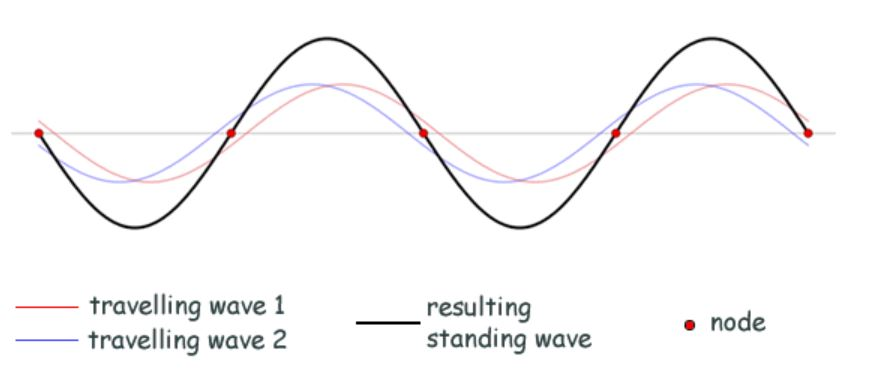
\includegraphics[height=5cm, width=10cm]{QuestionOne.JPG}
        \end{center}
        Equation $\dfrac{\partial^2 f}{\partial z^2}=\dfrac{1}{v^2} \dfrac{\partial^2 f }{\partial t^2}$ from the textbook 
        is the classical \textbf{wave equation}. Let's see if the given standing wave satisfies the wave equation. We define 
        $f(z,t)=f(z-vt, 0)=g(z-vt)$ and $u \equiv z-vt$.
        \\
        \\
        $
          \begin{cases}
            \dfrac{\partial f}{\partial z}=Ak ~ cos(kvt) ~ cos(kz)
            \\
            \\
            \dfrac{\partial^2 f}{\partial z^2}=-Ak^2 ~ cos(kvt) ~ sin(kz) ~~~~ (A)
          \end{cases}
          \begin{cases}
            \dfrac{\partial f}{\partial t}=-Akv ~ sin(kz) ~ sin(kvt)
            \\
            \\
            \dfrac{\partial^2 f}{\partial t^2}=-A k^2 v^2 ~ sin(kz) ~ cos(kvt) ~~~~ (B)
          \end{cases}
        $
        \\
        \\
        \\
        Now let's plug in $(A)$ and $(B)$ into the wave equation.
        \\
        \\
        $
          (A)=\dfrac{1}{v^2} (B) \Longrightarrow -Ak^2 ~ cos(kvt) ~ sin(kz)=\dfrac{1}{v^2} \times -A k^2 v^2 ~ sin(kz) ~ cos(kvt)
          \\
          \\
          \therefore ~~~ \boxed{cos(kvt) ~ sin(kz)=sin(kz) ~ cos(kvt)} ~~~~ \checkmark ~~~~ \emph{The wave equation is satisfied}
        $
        \\
        \\
        We are asked to express the given function as sum of a wave traveling to the left and a wave traveling to the right 
        according to $f(z,t)=g(z-vt)+h(z+vt) ~~ (\textbf{Eq. $9.6$})$. We know from trigonometry the below identity that we
        can use to rewrite $f(z,t)=A sin(kz) ~ cos(kvt)$.
        \\
        \\
        $
          \boxed{sin(\alpha) ~ cos(\beta)=\dfrac{1}{2} \left[sin(\alpha+\beta)+cos(\alpha-\beta)\right]}
          \\
          \\
          f(z,t)=A ~ sin(kz) ~ cos(kvt)=A \times \dfrac{1}{2} \left[sin(kz+kvt)+cos(kz-kvt)\right]
          \\
          \\
          \\
          \therefore ~~~ \boxed{f(z,t)=\dfrac{A}{2} ~ sin(kz+kvt)+\dfrac{A}{2} ~ cos(kz-kvt)=g(z-vt)+h(z+vt)} ~~~~ \checkmark
          \\
        $
      }

    \item \textbf{(9.4. 20 pts)} Obtain Eq. 9.20 directly from the wave equation, by separation of variables.

      % \textcolor{hwColor}{
      %   \\
      % }

    \item \textbf{(9.33. 30 pts)} The “inversion theorem” for Fourier transforms states that
    $$
      \tilde{\phi}(z)=\int\limits_{-\infty}^{+\infty} \tilde{\Phi}(k) ~ e^{ikz} ~ dk 
      \Longleftrightarrow 
      \tilde{\Phi}(k)=\dfrac{1}{2 \pi} \int\limits_{-\infty}^{+\infty} \tilde{\phi}(z) ~ e^{-ikz} ~ dz 
    $$
    Use this to determine $\tilde{A}(k)$, in $Eq. 9.20$, in terms of $f(z, 0)$ and $\dot{f}(z,0)$.

    [\emph{Answer:} $(1/2 \pi) \int\limits_{-\infty}^{+\infty} \left[
      f(z, 0)+(i/\omega) \dot{f}(z,0)
    \right]e^{-ikz} dz$]

      % \textcolor{hwColor}{
      %   \\
      % }

    \item \textbf{(9.35. 30 pts)} Suppose
    $$
      E(r, \theta, \phi, t)=A \dfrac{sin(\theta)}{r} \left[
        cos\left(kr-\omega t\right)-\left(1/kr\right) sin\left(kr-\omega t\right)
      \right] \hat{\phi}, ~~~ \text{with} ~ \dfrac{\omega}{k}=c
    $$
    (This is, incidentally, the simplest possible \textbf{spherical wave}. For notational convenience, 
    let $\left(kr-\omega t\right) \equiv u$ in your calculations.)
    \begin{enumerate}
      \item Show that $E$ obeys all four of Maxwell’s equations, in vacuum, and find the
      associated magnetic field.

        % \textcolor{hwColor}{
        %   \\
        % }

      \item Calculate the Poynting vector. Average $S$ over a full cycle to get the intensity
      vector $I$. (Does it point in the expected direction? Does it fall off like $r^{−2}$, as it
      should?)

        % \textcolor{hwColor}{
        %   \\
        % }

      \item Integrate $I.da$ over a spherical surface to determine the total power radiated.
      
      [\emph{Answer:} $4 \pi A^2/3 \mu_0 c$]

        % \textcolor{hwColor}{
        %   \\
        % }

    \end{enumerate}

  \end{enumerate}

\end{document}
